\documentclass[11pt,a4paper]{article}

\usepackage{iftex}

\ifpdftex
  \usepackage[utf8]{vietnam}
  \usepackage{tgpagella}
  \usepackage{amsmath, amssymb}
\else
  \usepackage{fontspec}
  \usepackage{unicode-math}
  \setmainfont{texgyrepagella-regular.otf}[
      BoldFont = texgyrepagella-bold.otf,
      ItalicFont = texgyrepagella-italic.otf,
      BoldItalicFont = texgyrepagella-bolditalic.otf
  ]
  \setmathfont{texgyrepagella-math.otf}
  \usepackage{amsmath}
\fi

\usepackage[a4paper, margin=2.5cm]{geometry}
\usepackage{graphicx}
\graphicspath{{images/}{src/dethi/images/}{src/dethi/latex/images/}}
\usepackage{microtype}
\usepackage{titlesec}
\usepackage{enumitem}
\usepackage{tikz}
\usetikzlibrary{arrows.meta}

% Căn chỉnh khoảng cách theo chuẩn quy định
\linespread{1.05}
\setlength{\parindent}{0pt}
\setlength{\parskip}{5pt plus 2pt minus 1pt}

% Khoảng cách hiển thị công thức toán
\setlength{\abovedisplayskip}{5pt plus 2pt minus 2pt}
\setlength{\belowdisplayskip}{5pt plus 2pt minus 2pt}
\setlength{\abovedisplayshortskip}{3pt plus 1pt}
\setlength{\belowdisplayshortskip}{3pt plus 1pt}

% Định dạng tiêu đề câu hỏi
\titleformat{\section}
  {\large\bfseries}
  {\thesection}{0.5em}{}
\titlespacing*{\section}
  {0pt}{8pt plus 2pt minus 1pt}{3pt plus 1pt minus 1pt}

\pagestyle{plain}

\begin{document}

\begin{center}
    {\Large\bfseries ĐỀ KIỂM TRA CUỐI KỲ 20231}\\[0.15cm]
    {\bfseries MÔN: VẬT LÝ ĐIỆN TỬ (PH3330)}\\[0.1cm]
    \textit{Đề số 2 --- Thời gian làm bài: 90 phút --- (Không sử dụng tài liệu)}
\end{center}
\vspace{0.1cm}

%=====================================================================
% CÂU 1
%=====================================================================
\section*{Câu 1. Chuyển động của điện tử trong ống tia điện tử}

Trình bày chuyển động của chùm điện tử trong ống tia điện tử dùng tụ điện lái tia như hình vẽ, biểu thức xác định độ nhạy của ống tia.

\begin{center}
    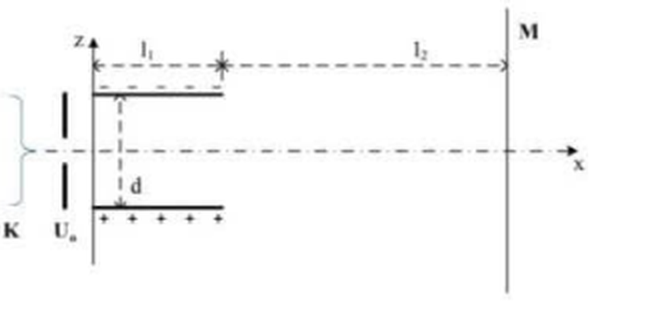
\includegraphics[height=2.6cm]{images/fig_20231_2.png}
\end{center}

%=====================================================================
% CÂU 2
%=====================================================================
\section*{Câu 2. Động học tương đối tính của điện tử}

Hạt điện tử được gia tốc bởi hiệu điện thế $U$ sao cho năng lượng toàn phần của điện tử gấp $3$ lần năng lượng nghỉ $E_0$ của nó.

\begin{enumerate}[label=\alph*., leftmargin=*, topsep=2pt, itemsep=1pt, parsep=0pt]
    \item Tính hiệu điện thế cần gia tốc cho điện tử.
    \item Tính vận tốc của điện tử.
    \item Tính khối lượng chuyển động của điện tử.
    \item Tính bước sóng De Broglie của điện tử.
\end{enumerate}

Cho biết: $E_0 = 511\text{ keV}$; $c = 3 \cdot 10^8\text{ m/s}$; $h = 6{,}625 \cdot 10^{-34}\text{ J}\cdot\text{s}$; $1\text{ eV} = 1{,}6 \cdot 10^{-19}\text{ J}$; $h \cdot c = 12{,}4 \cdot 10^3\text{ eV}\cdot\text{\AA}$.

%=====================================================================
% CÂU 3
%=====================================================================
\section*{Câu 3. Điện tử trong giếng thế năng một chiều}

Một điện tử bị nhốt trong giếng thế năng có vách vô cực có bề rộng của hố thế bằng $a$. Khi điện tử chuyển từ mức lượng tử thứ 5 xuống mức lượng tử thứ 2 bức xạ ra photon có năng lượng $10\text{ eV}$. Biết khối lượng của điện tử là $9{,}1 \cdot 10^{-31}\text{ kg}$; $1\text{ eV} = 1{,}6 \cdot 10^{-19}\text{ J}$; hằng số Planck $h = 6{,}625 \cdot 10^{-34}\text{ J}\cdot\text{s}$.

\begin{enumerate}[label=\alph*., leftmargin=*, topsep=2pt, itemsep=1pt, parsep=0pt]
    \item Xác định chiều rộng $a$ của giếng thế năng.
    \item Xác định vận tốc nhỏ nhất của điện tử trong giếng thế.
\end{enumerate}

%=====================================================================
% CÂU 4
%=====================================================================
\section*{Câu 4. Cấu trúc vùng năng lượng và tiếp xúc p-n}

Một mẫu bán dẫn tinh khiết có bề rộng vùng cấm $\Delta E_g = 1{,}0\text{ eV}$; ở nhiệt độ $300\text{ K}$ (ứng với $kT$ bằng $0{,}026\text{ eV}$) có nồng độ hạt dẫn riêng $n_i = 5 \cdot 10^{10}\text{ cm}^{-3}$ và mật độ trạng thái hiệu dụng $N_c = 4N_v$. Mẫu được pha tạp acceptor đồng đều trong toàn bộ mẫu với nồng độ $N_a = 1 \cdot 10^{14}\text{ cm}^{-3}$.

\begin{enumerate}[label=\alph*., leftmargin=*, topsep=2pt, itemsep=1pt, parsep=0pt]
    \item Tính mật độ trạng thái hiệu dụng $N_c$, $N_v$.
    \item Tính nồng độ điện tử, nồng độ lỗ trống, vị trí mức Fermi của mẫu bán dẫn.
    \item Nếu một nửa mẫu bán dẫn trên tiếp tục được pha tạp thêm tạp chất donor với nồng độ $1 \cdot 10^{16}\text{ cm}^{-3}$, hãy tính nồng độ điện tử, nồng độ lỗ trống, vị trí mức Fermi trong nửa mẫu này.
    \item Vẽ sơ đồ vùng năng lượng tại điều kiện cân bằng và tính hàng rào thế năng của điện tử giữa hai phần của cấu trúc sau khi nửa mẫu được pha tạp như ở câu c.
\end{enumerate}

\end{document}
